\section{SA³: Semantic Activity Annotation Algorithm}
\label{sec:clustering:sa3}

The objective of the $SA^3$ algorithm is to find sequences of actions that are describing an activity in an unlabelled sensor activation dataset. For that purpose, initial activity models (IAM) stored in the context knowledge are used. Remember that IAMs, as defined in definition \ref{def-iam}, are characterised by a sequence of necessary actions to perform an activity plus a duration estimation. 

The problem can be stated more formally as:

\begin{problem}[$SA^3$]
\label{prob-sa3}
 Given a context knowledge file where activities, sensors and objects are described and an unlabelled sensor activation dataset, find the occurrences of IAMs that form valid executions of activities.
\end{problem}

Considering that IAMs are sequences of actions and that sensor activation datasets are sensor sequences, Problem \ref{prob-sa3} can be seen as a pattern recognition problem, where IAMs act as the patterns to be recognised in the sensor activation dataset. Although $SA^3$ is actually a pattern recognition algorithm, there are some important features that make the problem special:

\begin{enumerate}
 \item IAMs are sequences of actions, whereas sensor activation datasets contain sensor activations, i.e. the activation of a concrete sensor of the environment.
 \item As IAMs are incomplete activity models, a user will generally execute more actions than those considered in the IAMs to perform activities. As a consequence a sensor activation dataset will generally include sensor activations and actions that are interleaved with IAM actions for the same activity.
 \item IAMs have no information about the order in which actions are executed, thus if $IAM(A) = \{a, b, c\}$, a sensor activation dataset containing the sequence $\{c, a, b\}$ has to be identified as activity $A$, i.e. the elements of the pattern to be recognised might appear in varied orders.
 \item Even though a sequence corresponding to an IAM is found, it does not necessarily describe a valid activity, since duration and location are important. For example, for an activity whose typical duration is 5 minutes, corresponding actions are found but their distance is of 3 hours; it is then common sense to think that those actions do not form a valid activity. Hence, the pattern recognition algorithm needs to take action time distances and locations into account.
 \item Sensors are prone to errors and in consequence, sensor activation datasets contain noise. The pattern recognition algorithm has to work thus in noisy environments. More concretely, considered kinds of sensor noise are positive and missing sensor noise (definitions \ref{def-positive} and \ref{def-missing}).
\end{enumerate}

In summary, $SA^3$ has to use IAMs as patterns to be recognised in an unlabelled sensor activation dataset, where actions are executed in varied orders, where actions that are not in IAMs can appear interleaved, where duration and location information is crucial for the validity of a pattern and where sensor noise exists. 

In order to tackle Problem \ref{prob-sa3} a three-step algorithm has been designed and implemented (see Figure \ref{fig:sa3_algorithm}). The first step, named sensor-action transformation step, uses sensor information from the context knowledge to transform sensor activations into actions (Section \ref{subsec:clustering:sa3:transform}). The second step, the activity sequence finding step, runs a pattern recognition algorithm using IAMs and object information from context knowledge, as described in Section \ref{subsec:clustering:sa3:find}. This step addresses the varied order of actions, interleaved actions not pertaining to IAMs, duration and location information for valid activities and sensor noise. Finally, the third step called correct activity sequence fitting fixes the overlapping activities generated in the second step (Section \ref{subsec:clustering:sa3:fit}).

\begin{figure}[htbp]
\centering
\includegraphics[width=\textwidth]{sa3_algorithm.pdf}
    \caption{The three-step algorithm for $SA^3$.}
    \label{fig:sa3_algorithm}
\end{figure}

The result of $SA^3$ is the partially annotated dataset. $SA^3$ can only label those actions pertaining to IAMs and thus it cannot infer a label for all the other actions of the sensor activation dataset. An example of how a partially annotated dataset looks like is provided in Table \ref{tab-partially-annotated}. The first column shows the timestamp of the sensor activation. The second column shows the activated sensor. Those two columns form the sensor activation dataset. $SA^3$ adds the third, fourth and fifth columns, where action, activity label and start/end tags are provided. Start tag refers to the first action pertaining to the IAM of a valid activity discovered by $SA^3$. End tag has the same meaning but for the last action. In consequence, start and end tags show the start and end times for a detected activity. For convenience, and even though any action not pertaining to the IAM of the detected activity cannot be labelled by $SA^3$, all the actions between start and end times are labelled with the detected activity name, and not with the special label None. This labelling criterion is applied to make visualization easier and it does not have any effect on the output of $SA^3$, neither for $AC$ nor for evaluation purposes.

\begin{comment}
\begin{figure}[htbp]
\begin{scriptsize}
\begin{lstlisting}
2014-05-23 07:42:17.106962,wsugarSens,hasFlavour,None,
2014-05-23 07:49:17.310460,bedSens,useFurniture,None,
2014-05-23 09:43:44.128079,cupSens,hasContainer,MakeChocolate,start
2014-05-23 09:47:33.984341,storeSens,openStore,MakeChocolate,
2014-05-23 09:47:39.333528,potSens,useCookingUtensil,MakeChocolate,
2014-05-23 09:47:52.750216,cookerSens,useCookingAppliance,MakeChocolate,
2014-05-23 09:48:07.764138,fridgeSens,openFridge,MakeChocolate,
2014-05-23 09:48:12.591836,wmilkSens,hasMilk,MakeChocolate,
2014-05-23 09:48:47.199512,chocoSens,hasChocolate,MakeChocolate,end
2014-05-23 09:54:11.553695,mugSens,hasContainer,None,
\end{lstlisting}
\end{scriptsize}
\caption{Example of a partially annotated dataset, the output of the $SA^3$ algorithm.}
\label{fig-partially-annotated}
\end{figure}
\end{comment}

\begin{table}[htbp]\scriptsize
  \begin{center}
        \begin{tabular}{ccccc}
            \hline            
            Timestamp & Sensor & Action & Activity & Start/End \\             
            \hline
            2014-05-23 07:42:17.106962 & wsugarSens & hasFlavour & None & \\
	    2014-05-23 07:49:17.310460 & bedSens & useFurniture & None & \\
	    2014-05-23 09:43:44.128079 & cupSens & hasContainer & MakeChocolate & start \\
	    2014-05-23 09:47:33.984341 & storeSens & openStore & MakeChocolate & \\
	    2014-05-23 09:47:39.333528 & potSens & useCookingUtensil & MakeChocolate & \\
	    2014-05-23 09:47:52.750216 & cookerSens & useCookingAppliance & MakeChocolate & \\
	    2014-05-23 09:48:07.764138 & fridgeSens & openFridge & MakeChocolate & \\
	    2014-05-23 09:48:12.591836 & wmilkSens & hasMilk & MakeChocolate & \\
	    2014-05-23 09:48:47.199512 & chocoSens & hasChocolate & MakeChocolate & end \\
	    2014-05-23 09:54:11.553695 & mugSens & hasContainer & None & \\
            \hline
        \end{tabular}                
        \caption{Example of a partially annotated dataset, the output of the $SA^3$ algorithm shown in table format.}
        \label{tab-partially-annotated}
    \end{center}
\end{table}

The next sections describe in detail the three steps of $SA^3$ depicted in Figure \ref{fig:sa3_algorithm}. Finally, Section \ref{subsec:clustering:sa3:complete} shows the complete algorithm and illustrates it with an example.
% Note: The following two paragraphs can be used in summary and conclusions?
%Real-time activity recognition needs complete activity models to have a reliable recognition performance. However, providing complete activity models is very complicated, since each user executes varied action sequences to perform the same activity. For example, to make a coffee, some users may use milk and sugar, while others may add only some cream. But making coffee will always imply using coffee and having a container, i.e. the action sequence \textit{\{hasContainer(x), hasCoffee(y)\}}. This prior knowledge is used in $SA^3$ for activity annotation.

%Activity annotation and recognition is not the same thing. Activity annotation can make use of the whole dataset offline, with no time restrictions. On the other hand, activity recognition is required to work while activities are being performed, so only past sensor activations can be used. This key difference makes feasible using incomplete activity models to annotate activities, in contrast with the real-time recognition problem.

\subsection{Sensor-action transformation step}
\label{subsec:clustering:sa3:transform}

The first step takes as inputs the sensor activation dataset and the context knowledge file to transform every sensor activation into an action. For each sensor activation in the dataset, the corresponding sensor model is checked in the context knowledge file. As shown in Figure \ref{fig-context-json} every sensor has the action to which it has to be mapped in the context knowledge file provided by the domain expert. This simple transformation is possible due to the dense sensing-based activity monitoring approach, where sensor activations are directly linked to user-object interactions and thus to actions. 

In consequence, a sensor activation sequence such as:
 \begin{equation*}
 \begin{split}
   \{cupSens, wsugarSens, smilkSens\}
 \end{split}  
 \end{equation*}
 will be transformed to:
 \begin{equation*}
 \begin{split}
  \{hasContainer(cup), hasFlavour(white\text{-}sugar), hasMilk(skimmed\text{-}milk)\}
 \end{split}   
 \end{equation*}
 
For the sake of clarity, and given that action matching does not care about concrete objects used to execute that action, \textit{hasContainer(cup)} will be used as \textit{hasContainer}. But notice that the object information obtained through the sensor activation is not removed. 

Sensor-action transformation step allows performing pattern recognition in the action space, abstracting from concrete sensor activations. This step can be kept simple thanks to the dense sensing-based approach. For different activity monitoring approaches, such as wearable sensors, more complex sensor-action transformation steps should be implemented. However, notice that as far as sensor information can be transformed to actions, $SA^3$ and the entire clustering process can work without any problem. This is why constraint \ref{cons-dense} is considered to be a weak constraint.

\subsection{Activity sequence finding step}
\label{subsec:clustering:sa3:find}

The objective of this step is to find all valid occurrences of IAMs in the action space obtained from the sensor-action transformation step. An iterative process is run over actions. Firstly, the algorithm checks whether current action pertains to any of the IAMs stored in the context knowledge file. If the answer is no, the action is labelled with the None label and the next action is treated. But if the answer is yes, the IAMs of the activities in which the action appears are considered as possible activities. Notice that if the action pertains to more than one IAM, all the possibilities are treated. Assume the action $a$ pertains to $IAM(A_1)$ and $IAM(A_2)$. Two action sequences are created $S(A_1) = \{a\}$ and $S(A_2) = \{a\}$. The algorithm iterates through the next actions, in order to find sequences of actions that form valid activities in correspondence of possible activities.

The process to find valid activities works as follows:

\begin{enumerate}
 \item Current action $b$ is added to the created action sequences: $S(A_i) = append(S(A_i), b)$.
 \item If current action $b$ pertains to an IAM of an activity for which no sequence has been open, open a new sequence.
 \item Check whether candidate sequences form a valid activity in terms of \textit{completion}, \textit{duration} and \textit{location}
 \item If any of the candidate sequences forms a valid activity, close the sequence and follow with remaining sequences.
 \item Iterate through actions until all sequences are closed (valid activities) or removed (invalid activities).
\end{enumerate}

To fully understand the described process to check for valid activities, the \textit{completion}, \textit{duration} and \textit{location} criteria have to be explained:

\begin{enumerate}
  \item Completion criterion: an action sequence has to contain all the actions of the corresponding IAM to be considered a complete action sequence for the corresponding activity. An action sequence $S(A_i)$ is complete for activity $A_i$ if and only if 
  \begin{equation}
  \label{eq-completion}
  IAM(A_i) \subseteq S(A_i)   
  \end{equation}
  
  \item Duration criterion: for an action sequence to fulfil the duration criterion, the duration of the action sequence has to be smaller than the duration estimation of the corresponding IAM. The duration of an action sequence $S(A_i)$ is calculated as the rest of the timestamps of the last action and the first action: 
  \begin{equation}
    \Delta_t(S(A_i)) = t(S(A_i)_{last}) - t(S(A_i)_{first})
  \end{equation}
  where $t(S(A_i)_j)$ is the timestamp of the $j$-th action of the sequence $S(A_i)$. Duration estimations for activities are stored in the context knowledge file and are written as $\Delta_t(A_i)$. Hence, the duration criterion establishes that an action sequence fulfils the duration criterion if and only if 
  \begin{equation}
   \label{eq-duration}
   \Delta_t(S(A_i)) \leq \Delta_t(A_i)
  \end{equation}  
  
  \item Location compatibility criterion: the actions of sequence $S(A_i)$ which pertain to $IAM(A_i)$ have been transformed from corresponding sensor activations. Those sensor activations can be traced in the context knowledge to the used objects. And those objects have a location in their model. Hence, the location of actions can be inferred using the context knowledge file. Using this information, the location of the possible activity described by sequence $S(A_i)$ is inferred. The location of sequence $S(A_i)$ is inferred as the common locations of actions of the sequence pertaining to $IAM(A_i)$. If actions pertaining to the IAM do not share a common location, the sequence has no location and thus, it is not location compatible with any activity. On the other hand, if a common location is shared, that location has to be compatible with the locations of the corresponding activity, modelled in the context knowledge file. Notice that only locations of actions pertaining to an IAM are considered. All the other actions can be generated by noise or erratic behaviour and in consequence, their locations are not considered in $SA^3$.
 \end{enumerate}

Action sequences that fulfil the completion, duration and location criteria will be considered as valid activities and stored as such. Action sequences that do not fulfil those criteria will be removed, since they do not form a valid activity description.  

\subsection{Correct activity sequence fitting step}
\label{subsec:clustering:sa3:fit}
Depending on the activity models, the sensor activation dataset and noise levels, valid activities can overlap each other. Moreover, as many IAMs will share some actions, activity overlapping will be a normal scenario after activity sequence finding step described in Section \ref{subsec:clustering:sa3:find}. But by virtue of constraint \ref{cons-single}, interleaving thus overlapping activities cannot appear in the sensor activation dataset. So a special step has to be designed to treat overlapping activities generated in the activity sequence finding step. 

Having a set of overlapping activities, described through corresponding action sequences, this step introduces a heuristic directly derived from constraint \ref{cons-single} to return a set of non-overlapping activities which provides the best explanation for the generated situation. The heuristic states that in a set of overlapping action sequences, the maximum number of non-overlapping action sequences have to be returned. 

The reason to adopt this heuristic is that the vast majority of sensor activations are originated by deliberated user-object interactions. In consequence, the vast majority of sensor activations must be part of an activity. In order to maximise the number of sensor activations which correspond to the execution of an activity, the heuristic chooses the maximum number of non-overlapping activities in a given sequence. Because this is the way to maximise the number of sensor activations in activities.
 

\subsection{The complete SA³ algorithm}
\label{subsec:clustering:sa3:complete}

Sections \ref{subsec:clustering:sa3:transform}, \ref{subsec:clustering:sa3:find} and \ref{subsec:clustering:sa3:fit} describe the first, second and third steps of the $SA^3$ algorithm. This three-step algorithm is depicted as pseudo-code in Algorithm \ref{alg:sa3}. It has been designed to work with noisy sensor activations, varying order for activity executions and sensor activations that do not belong to any initial activity model. That flexibility allows using the tool in many different datasets. 

\begin{algorithm}
 \caption{$SA^3$ algorithm for semantic activity annotation}
 \label{alg:sa3}
 \begin{algorithmic}
 \REQUIRE sensor\_activation\_dataset, context\_knowledge
 \ENSURE partially\_annotated\_dataset
 \STATE $partially\_annotated\_dataset \leftarrow createDataset(sensor\_activation\_dataset)$
 \STATE $action\_dataset \leftarrow applyTransformFunction(sensor\_activation\_dataset,$ 
 $context\_knowledge)$
 \STATE $IAM\_list \leftarrow obtainIAMS(context\_knowledge)$
 \FORALL{$action \in action\_dataset$}
  \IF{$action \in initial\_activity\_models$}
    \STATE $activities \leftarrow obtainActivities(action, IAM\_list)$
  \ENDIF
  \FORALL{$activity \in activities$}
    \STATE $// \text{ Use duration, completion and location criteria}$
    \STATE $valid\_activities \leftarrow findValidActivities(context\_knowledge)$
  \ENDFOR
 \ENDFOR
 \STATE $partially\_annotated\_dataset \leftarrow findNonOverlappingActivities(valid\_activities)$
 \RETURN $partially\_annotated\_dataset$
 \end{algorithmic}
\end{algorithm}

An illustrative example is shown next, to describe how $SA^3$ works. Time-stamps are ignored in the example, considering that duration criterion is fulfilled by the shown action sequence and considered activities. This assumption helps making the example clearer. The illustrative example has been designed to show in detail how $SA^3$ works, so it does not have to be coherent with the reality. 

Imagine initial activity models for MakeCoffee, MakeTiramisu, MakeWhippedCream and BrushTeeth are defined as follow:
 \begin{equation*}
  \begin{split}
  MakeCoffee =\{hasCoffee, hasContainer, hasFlavour\} \\
  MakeTiramisu = \{hasCream, hasContainer, hasCoffee\} \\
  MakeWhippedCream = \{hasFlavour, hasContainer, hasCream\} \\
  BrushTeeth = \{hasBrusher, hasToothPaste, turnOnTap\} 
  \end{split}
 \end{equation*} 
 
Notice that there are many actions that are used for the IAMs of several activities. For instance, \textit{hasContainer} is used in the IAMs of MakeCoffee, MakeTiramisu and MakeWhippedCream. Using the same actions for various activities makes the problem harder, since overlapping activities are more common.

Let us consider the following sensor activation sequence from the sensor activation dataset:

\begin{equation*}
\begin{split}
 \{mugSens, creamSens, spoonSens, whitesugarSens, brusherSens, \\ 
 afcoffeeSens, toothpasteSens, glassSens, btapSens\}
\end{split}  
\end{equation*}

Applying the sensor-action transformation step using the context knowledge as described in Section \ref{subsec:clustering:sa3:transform}, the following action sequence is obtained (concrete objects are ignored in the action sequence):

\begin{equation*}
\begin{split}
 \{hasContainer, hasCream, useCookingUtensil, hasFlavour, hasBrusher, \\ 
 hasCoffee, hasToothpaste, hasContainer, turnOnTap\}
\end{split}  
\end{equation*}

Figure \ref{fig:overlap-l} shows all the activities found by the second step of $SA^3$ (Section \ref{subsec:clustering:sa3:find}). Activities overlap each other, because there are several actions that belong to several activities. Notice also that there are some actions that are not in any activity model, which is totally feasible for the approach.

\begin{figure}[htbp]
 \begin{small}
\begin{lstlisting}
 hasContainer      |     |
 hasCream          | MWC |
 useCookingUtensil |     |
 hasFlavour        |     | MT 
 hasBrusher              |    |
 hasCoffee               |    |
 hasToothpaste                | BT
 hasContainer                 |
 turnOnTap                    |
\end{lstlisting}
\caption{Illustrative example of the output of the activity sequence finding step of $SA^3$. MWC refers to MakeWhippedCream, MT to MakeTiramisu  and BT to BrushTeeth.}
\label{fig:overlap-l}
\end{small}
\end{figure}

Assuming duration criterion is always fulfilled for this example, Figure \ref{fig:overlap-l} shows how the completion and location criteria work. For instance, action sequence $S = \{hasContainer, hasCream, useCookingUtensil, hasFlavour\}$ is a valid sequence to describe activity MakeWhippedCream, because it contains all the actions of $IAM(MakeWhippedCream)$ and it is location compatible. Actions \textit{hasContainer, hasCream} and \textit{hasFlavour}, which pertain to $IAM(MakeWhippedCream)$ are obtained by interacting with objects \textit{mug, cream} and \textit{white-sugar}. The location of all those objects is the kitchen. As activity location for MakeWhippedCream is set to kitchen, the action sequence and the activity are location compatible.

However, consider the following action sequence $S = \{$ $hasFlavour,$ $hasBrusher,$ $hasCoffe,$ $hasToothpaste,$ $hasContainer\}$. Assuming duration criterion is satisfied, it can be seen that the completion criterion is also satisfied for activity MakeCoffee. But sequence $S$ does not form a valid activity because the last action \textit{hasContainer} is produced by the object \textit{glass}, which is located in the bathroom. As \textit{hasContainer} is in $IAM(MakeCoffee)$, its location is taken into account for location inference and compatibility. In this case, sequence $S$ does not have a unique location and hence, it is removed. 

After activity sequence finding step finishes, three overlapping valid activities are found, namely MakeWhippedCream, MakeTiramisu and BrushTeeth. Such a situation cannot happen in a single user - single activity scenario, so the third step has to be applied: correct activity sequence fitting step (Section \ref{subsec:clustering:sa3:fit}). Using the defined heuristic, two activities are returned:

\begin{equation*}
  \begin{split}   
  MakeWhippedCream = \{hasContainer, hasCream, useCookingUtensil,\\ 
  hasFlavour\} \\
  BrushTeeth = \{hasBrusher, hasCoffee, hasToothPaste, hasContainer,\\ 
  turnOnTap\} 
  \end{split}
 \end{equation*} 

Those two activities are the maximum number of non-overlapping activities found in the set of valid activities. The action sequence for MakeWhippedCream makes perfect sense. There is an action, \textit{useCookingUtensil}, which is not in any IAM, but it is very coherent with the activity. Even though $SA^3$ labels this action with the MakeWhippedCream tag, remember there is no way for $SA^3$ to know whether this action is really part of the activity. Such a labelling is done only for convenience. On the other hand, the action sequence for activity BrushTeeth contains a strange action: \textit{hasCoffee}. In a noisy scenario this action may be generated by sensor or communication infrastructure errors. The other action which is not in the IAM of BrushTeeth is \textit{hasContainer}. It is generated by the \textit{glass} sensor, which is located in the bathroom. Action \textit{hasContainer} may refer to a glass used in the bathroom to rinse the mouth. 

Looking at Figure \ref{fig:overlap-l}, the heuristic defined in the correct activity sequence fitting step can be visually understood. As it can be seen, returning the maximum number of non-overlapping activities maximises also the number of actions inside activities.